\documentclass[12pt]{article}
\usepackage[brazil]{babel}
\usepackage[a4paper,margin=2.5cm]{geometry}
\usepackage{graphicx}
\usepackage{minted}
\usepackage{setspace}
\usepackage{indentfirst}

\frenchspacing

\begin{document}

% ================= CAPA =================

\begin{titlepage}
    \centering

    % Logo UFMG
    \vspace*{1.5cm}
    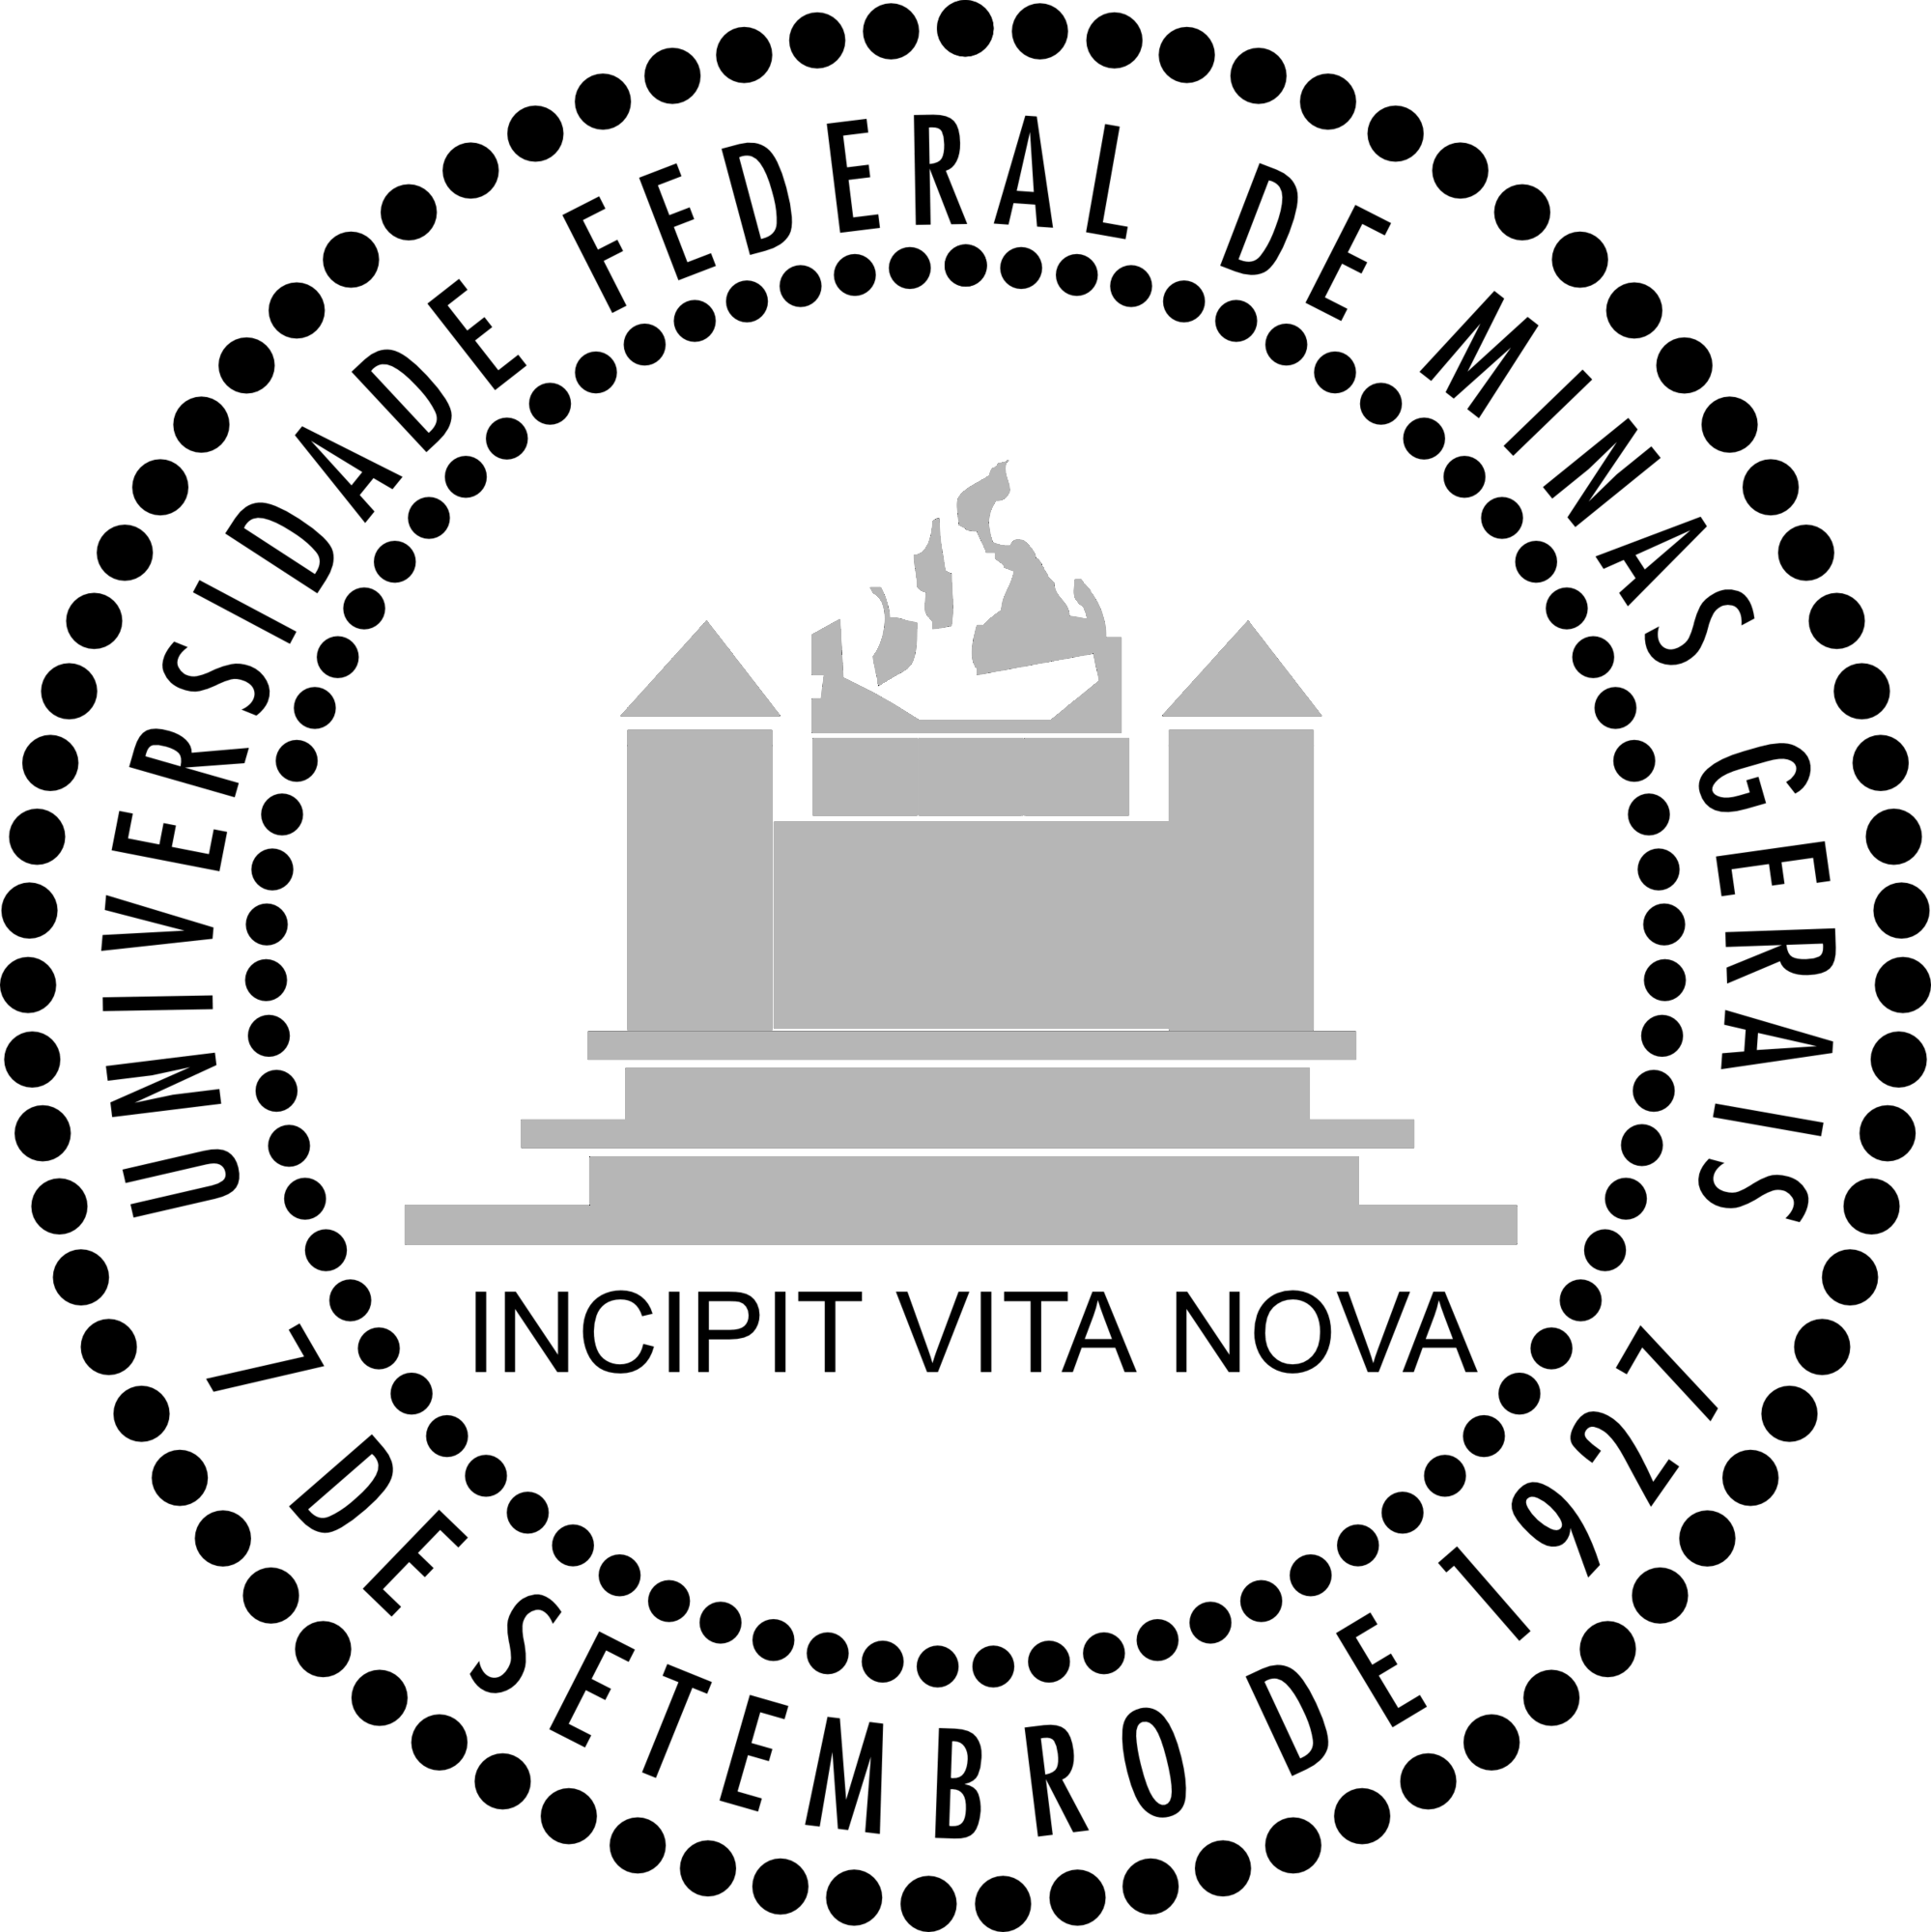
\includegraphics[width=4cm]{imagens/logo.png}

    \vspace{1.5cm}

    % Universidade
    {\LARGE
    \textbf{UNIVERSIDADE FEDERAL DE}\\[0.2cm]
    \textbf{MINAS GERAIS}
    }

    \vfill


    % Título
    {\huge
    \textbf{TRABALHO FINAL DE}\\[0.15cm]
    \textbf{AUTOMAÇÃO EM TEMPO REAL}
    }

    \vspace{0.8cm}

    {\Large Entrega 1: Definição da Arquitetura}

    \vfill

    % Integrantes
    {\large
    Ana Clara Melado, 2023421386 \\[0.3cm]
    Bruno Araujo Pinto, 2023038965\\[0.3cm]
    Mariana Villefort Rabelo, 2022061033
    }

    \vfill

    % Rodapé
    {\large
    Belo Horizonte \\[0.2cm]
    \today
    }

\end{titlepage}

% ================= CONTEÚDO =================

\section{Introdução}

\begin{figure}[ht]
  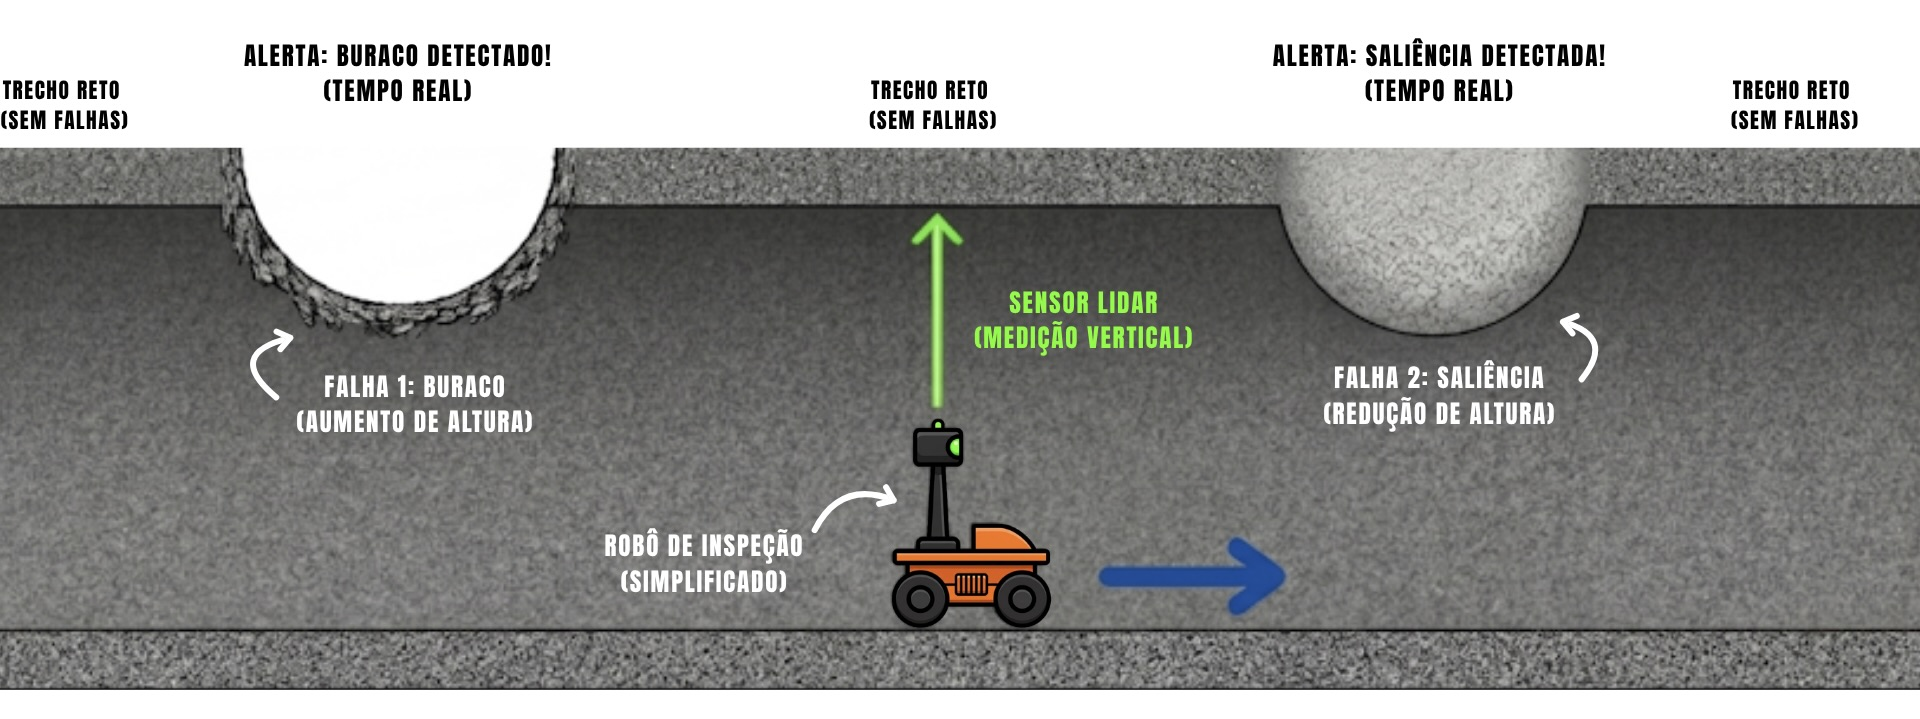
\includegraphics[ width= \linewidth]{imagens/introducao.jpeg}
  \caption{Tunel (vista lateral 2D)}\label{fig:introducao}
\end{figure}

A inspeção periódica de túneis e estruturas civis é fundamental para garantir a segurança operacional e estrutural desses ambientes. Entretanto, métodos tradicionais de inspeção manual apresentam limitações relacionadas ao custo, ao tempo de execução e à exposição de operadores a ambientes potencialmente perigosos. Nesse contexto, sistemas autônomos de inspeção vêm sendo cada vez mais utilizados, permitindo a coleta contínua de dados e a identificação precoce de falhas estruturais.

Este trabalho tem como objetivo o desenvolvimento da arquitetura de um sistema embarcado para inspeção automática de túneis, utilizando conceitos de Automação em Tempo Real, programação concorrente e sincronização entre tarefas. O sistema proposto simula o funcionamento de um robô autônomo responsável por percorrer um túnel realizando medições da superfície do teto por meio de sensores simulados, como encoder e LIDAR, possibilitando a detecção de irregularidades estruturais.

A implementação desenvolvida na primeira etapa do projeto concentra-se principalmente nas tarefas responsáveis pelo controle de navegação, cálculo de distância percorrida, reconstrução da superfície do túnel e coleta de dados. Para isso, foram utilizados processos e múltiplas threads em \texttt{C++}, além de mecanismos de sincronização como \texttt{mutex} e \texttt{condition\_variable}, garantindo acesso seguro aos buffers compartilhados e evitando condições de corrida durante a troca de informações entre produtor e consumidor.

Além da implementação dos buffers compartilhados, o projeto também realiza testes preliminares de sincronização e bloqueio, verificando situações de buffer vazio e buffer cheio. Esses testes permitem validar o comportamento concorrente do sistema e demonstrar a correta coordenação entre as tarefas executadas em paralelo, aspecto essencial em aplicações de tempo real.

Por fim, esta etapa do trabalho estabelece a base arquitetural necessária para as próximas implementações do sistema completo, incluindo comunicação remota, interface gráfica de operação e integração com protocolos de comunicação.

\section{Proposta de Arquitetura}

    A arquitetura do trabalho foi realizada com o intuito de facilitar o máximo possível
    a aplicação dos conceitos, por isso a utilização máxima de threads. A partir dos requisitos mínimos,
    pelo menos 2 processos foram criados. Além, aproveita-se das threads originárias dos póprios
    processos para evitar a criação desnecessária de mais threads. A arquitetura pode ser conferida na figura \ref{fig:arquitetura}.
\begin{figure}[ht]
  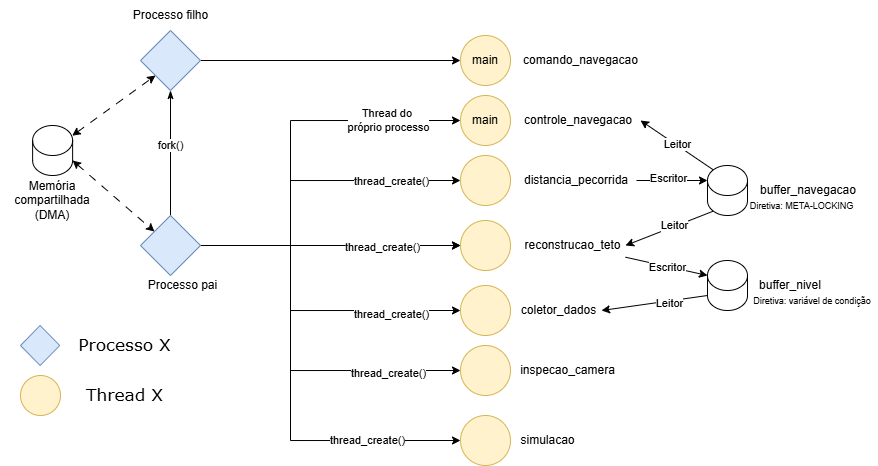
\includegraphics[ width= \linewidth]{imagens/arquitetura_threades_processos.png}
  \caption{Proposta de arquitetura para o trabalho prático. Losangos representam processos e círculos representam threads.}\label{fig:arquitetura}
\end{figure}

Ademais, para a comunicação e recursos compartilhados, foi utilizada uma diretiva diferente de sincronização. No caso do buffer\_navegacao,
 foi utilizado o método do META-LOCKING. Para o buffer\_nivel, foram utilizadas variáveis de condição,  de forma "normal". %chktex 18
  E por fim, a comunicação entre os processos foi feita por meio da memória compartilhada.

\section{Resultados de Testes Preliminares Realizados}

\section{Conclusão}

\section{Apêndice}
\section{Exemplo de Código}

\begin{minted}[
    linenos,
    breaklines,
    frame=lines,
    fontsize=\small
]{cpp}
#include <iostream>

int main() {
    std::cout << "Olá mundo!" << std::endl;
    return 0;
}
\end{minted}

\end{document}